Die Aufgabenstellung haben wir in folgende Teilaufgaben eingeteilt:
\begin{enumerate}
	\item Finden der möglichen Hautschuppen
	\item Filtern, welche der Hautschuppen tatsächlich zu einem Rhinozelfanten gehören
	\item Einfärben des gesamten Rhinozelfanten
\end{enumerate}

Eine Hautschuppe haben wir als Pixel definiert, das mehr als zwei gleichfarbige Nachbarfelder hat. Nachbarfelder sind alle direkt und diagonal anliegenden Pixel.

Diese Hautschuppenmenge enthält allerdings noch einige vermeintliche Hautschuppen, die zu keinem Rhinozelfanten gehören. Beispielsweise werden oft Pixel im Himmel fälschlich als Hautschuppe erkannt, da nur wenige Blautöne vorliegen. Diese False Positives müssen für ein besseres Ausgabebild herausgefiltert werden.

Dazu haben wir zuerst das Problem vereinfacht: Anstatt dies direkt auf dem bunten Bild durchzuführen, wird ein Schwarz-Weiß-Bild erstellt. In diesem Bild sind schwarze Pixel mögliche Hautschuppen, weiße Pixel sind auf keinen Fall Hautschuppen. Dieses Zwischenbild wird Ihnen in der GUI angezeigt.

Auf dieses werden folgende Filter angewandt, um zu bestimmen, welche möglichen Hautschuppen tatsächlich Teil eines Rhinozelfanten sind.

\begin{description}
	\item[Linienfilter] Zuerst wird nach ausreichend großen durchgehenden Linien gesucht: Einzelne Hautschuppen können schließlich keine Rhinozelfanten sein. Wir haben festgelegt, dass ein Rhinozelfant an seiner dicksten Stelle 4\% der Gesamtbreite des Bildes haben muss. Dies überschreiten alle Rhinozelfanten in den Beispielen deutlich. Kleinere Werte würden die Laufzeit erheblich verlängern, da mehr mögliche Rhinozelfanten an die nachfolgenden Filter weitergegeben werden würden. Größere Werte würden dementsprechend den Programmablauf beschleunigen, es könnten jedoch Rhinozelfanten übersehen werden. Alle Linien, die dieses Kriterium erfüllen, werden an den nächsten Filter weitergegeben.
	\item[Rechteckfilter] In den Bauch eines Rhinozelfanten lässt sich ein Rechteck zeichnen. In diesem Schritt wird überprüft, ob sich mit der soeben gefundenen Linie als obere Kante ein Rechteck höher als 1,25\% der Gesamthöhe des Bildes zeichnen lässt. Alle Rechtecke, die dieses Kriterium erfüllen, werden an den nächsten Filter weitergegeben.
	\item[Anatomiefilter] Zuletzt wird überprüft, ob sich das Umfeld des Rechteckes mit der Anatomie eines Rhinozelfanten deckt. Dazu wird überprüft, ob sich an das Rechteck Beine anzeichnen lassen. Auf den Rüssel wird nicht eingegangen, da seine Position stark variiert und die drei vorher genannten Filter keine False Positives gefunden haben.
\end{description}

Wenn von einer Stelle ausgehend sämtliche Kriterien zutreffen, sind alle zusammenhängenden Hautschuppen ein Rhinozelfant. Zwei Hautschuppen hängen zusammen, wenn sie benachbart sind.

\clearpage
Beispiel: \vspace{3em}
\begin{figure}[!ht]
	\centering
	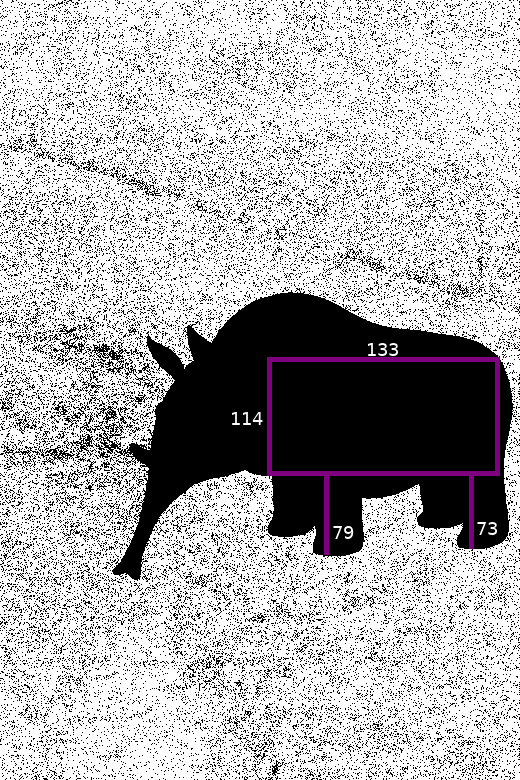
\includegraphics[width=0.7\textwidth]{SkizzeIdee4}
	\caption {Bsp. 4. mit eingezeichneten Skelett}
	Um den Filtereffekt zu verdeutlichen, wurde jedes Pixel mit mehr als einem gleichfarbigen Nachbar markiert.
\end{figure}
\clearpage

\subsection {Überlegungen zur Laufzeit}
Die Laufzeit des Programmes wächst ungefähr linear zu der Gesamtpixelzahl des Bildes, da der Großteil der Laufzeit für die Suche nach möglichen Hautschuppen und das Auszählen der Linienlängen genutzt wird.

Die Beschaffenheit (Anzahl möglicher Hautschuppen) spielt im Average-Case eine eher geringe Rolle, da die meisten Pixel bei der Hautschuppensuche und der Linienananlyse mit jeweils konstanter Laufzeit ausgeschlossen werden können.

Im Best-Case, also einem Bild aus zufälligem Rauschen, in dem keine Filter zum Einsatz kommen, benötigt das Programm für 6 Mio. Pixel (2000x3000) 2.3s. 
Wenn nun in einem Average-Case (Bsp. 4) einige Filterausführungen zum Finden eines im Bild vorhandenen Rhinozelfanten benötigt werden, steigt die Laufzeit marginal auf 2.6s an. 
Im Worst-Case, nämlich einem komplett einfarbigen Bild, in dem alle Pixel mögliche Hautschuppen sind, werden zahlreiche komplette Filterdurchläufe benötigt, die Laufzeit beträgt dann 30s.